
%This is the hello world document, it is very usefull
%As you can see the character % is used for comments

\documentclass[a4paper,12pt]{article}
%\documentclass[doc]{apa}
\usepackage[usenames,dvipsnames]{color}
\usepackage{graphicx}
\usepackage{multicol}
\usepackage{multirow}
\usepackage{amsmath}
\usepackage{hyperref}
\usepackage{pdfpages}

%\setlength\parindent{0pt}
%\usepackage{figure}
\usepackage[margin=0.8in]{geometry}
\title{Project 1. Content Based Image Retrieval Using Global and Local Features}
\author{Dan Bryan and Olmo Zavala}

\begin{document}
\maketitle

For this project three approaches for Content Based Image Retrieval  (CBIR)
where implemented. The first approach is based on the comparison of color 
histograms, the second solution uses spectral histogram to do the comparison
of images, and the third approach uses SIFT features to compare images. 

\section{Description}
In this section the three methods used for CBIR are described. 

\subsection{Color histogram}
\label{sec_colorhist}
In this method we used the color (intensity filter) histogram  to 
compare images. The following steps summarizes the method:
\begin{enumerate}
    \item \textbf{Image pyramidization. } The images sizes where reduced
        to half their size in order to speed up the algorithm. The method used
        to compute the pyramids is \emph{Gaussian pyramid}, the first
        step of the Gaussian pyramid algorithm is to blur the image 
        using a Gaussian filter, and then scale down the image by 
        creating one pixel from the average color of four pixels.
    \item \textbf{Compute histograms.} The number of bins used
        for this method is 256, for each color band.
    \item \textbf{Compute histogram distances.} The distance between
        each pair of image histograms were computed using histogram intersection:
        \begin{equation}
            dist(hist_a,hist_b) = \sum_{i=1}^{256} \min( hist_a(i), hist_b(i))
        \end{equation}
    \item \textbf{Images similarity}. The distance between the histograms
        of the images was used as the \emph{similarity} parameter. 
\end{enumerate}

\subsection{Spectral histogram}
\label{sec_spechist}
This method uses spectral histograms for CBIR. The proposed steps
for this method are the following:

\begin{enumerate}
    \item \textbf{Image pyramidization. } The images sizes where reduced
        to half their size in order to speed up the algorithm. The method used
        to compute the pyramids is \emph{Gaussian pyramid}, the first
        step of the Gaussian pyramid algorithm is to blur the image 
        using a Gaussian filter, and then scale down the image by 
        creating one pixel from the average color of four pixels.
    \item \textbf{Filter images}. Six filters plus the intensity
        filter are applied to each of the images. The filters 
        used and their corresponding masks are:
        \begin{equation}
            \begin{split}
                \frac{\partial I}{\partial x} & =  [0~-1~1] \\
                \frac{\partial I}{\partial y} & =  [0~-1~1]^T \\
                \frac{\partial I}{\partial x \partial x} & = [-1~2~-1] \\
                \frac{\partial I}{\partial y \partial y} & = [-1~2~-1]^T \\
                LoG(I(x,y))  & = ( x^2 + y^2 - \sqrt{2\sigma^2} ) e^{ -(x^2+y^2)/\sqrt{2\sigma^2}}\\
                Gauss(I(x,y))  & = \frac{1}{2 \pi \sigma^2} e^{ \frac{-(x.^2+y.^2)}{2\sigma^2}}\\
            \end{split}
        \end{equation}
        For the Laplacian of Gaussian (LoG) and Gaussian filters the size of the filter
        used is $5$ with a sigma value of $0.7$.
    \item \textbf{Compute spectral histograms.} The number of bins used
        for this method is 100, for each color band and for each filter. 
        For all the filters the range goes from [0 256], even when the values of some
        of the filters may go from [-256 256]. Several options for the range of the 
        histograms were tested, and the range of [0 256] gave the best results. 
        The 100 bins are evenly split from [0 256].
        Figure \ref{fig:spechist} shows an example of the spectral histograms. 
        \begin{figure}[h]
            \centering
            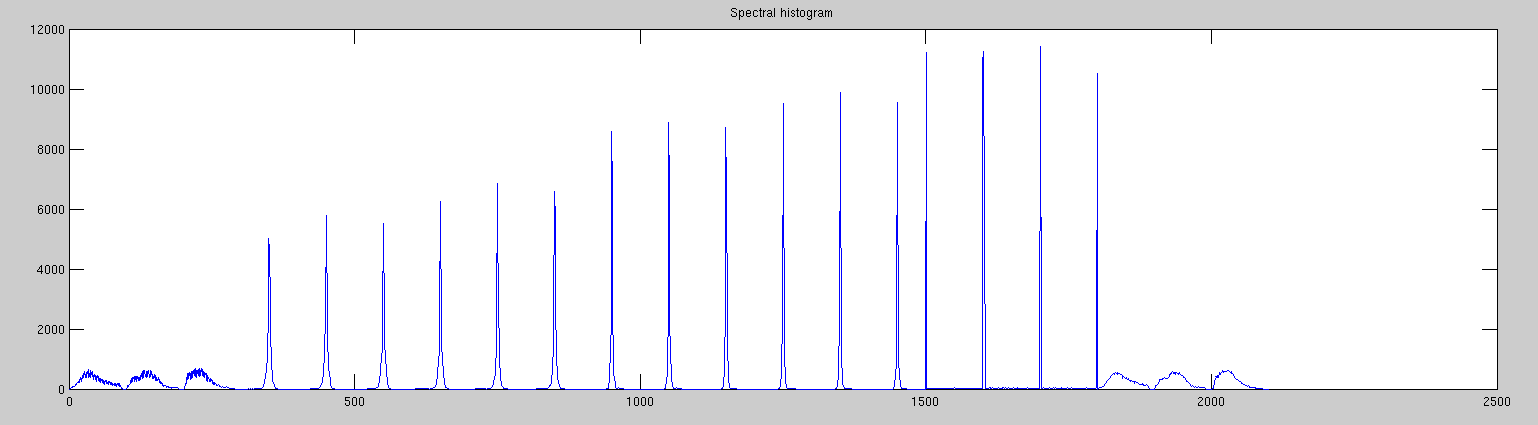
\includegraphics[totalheight=.18\textheight]{./Images/SpectralHist.png}
            \label{fig:spechist}
        \end{figure}
    \item \textbf{Compute histogram distances.} The distance between
        each pair of image histograms were computed using histogram intersection:
        \begin{equation}
            dist(hist_a,hist_b) = \sum_{i=1}^{100} \min( hist_a(i), hist_b(i))
        \end{equation}
    \item \textbf{Images similarity}. The distance between the histograms
        of the images was used as the \emph{similarity} parameter. 
\end{enumerate}

\subsection{SIFT Features}
For this method we use the SIFT descriptors to compare images. The code is based on  
the implementation provided at \url{http://www.vlfeat.org/}{vlfeat.org}. The proposed steps
to obtain a score that could be used for CBIR are:

\begin{enumerate}
    \item Obtain the SIFT descriptors for each image using function \textbf{vl\_sift}. 
    \item Compute the matching descriptors and the distance between those descriptors using
        the function \textbf{vl\_ubcmatch}.
    \item Obtain the maximum distance obtained between all the matches (for later normalization).
    \item Combine the average distance of the matched descriptors with the 
        number of matched descriptors between two images using \emph{Cantor pairing}. Equation \ref{eq:sift}
        show the score computed between images $i$ and $j$ using the SIFT features.
        \begin{equation}
            \begin{split}
                k1 & = mean( \frac{\text{matches}(i,j)}{\text{maxDist}})\\
                k2 & = \text{length}(\text{matches}(i,j)) ~ \text{\# matched descriptors}\\
                \text{siftScore}(i,j) & =  (0.5*(k1+k2)*(k1+k2+1))+k2
            \end{split}
            \label{eq:sift}
        \end{equation}
\end{enumerate}


\subsection{Computation time}
The three methods were implemented in parallel (when possible) using the
matlab function $parfor$. The third method, which uses SIFT features,
takes a lot more time than the others and the computation time is presented separated
at the end of this section. \\

For eficiency, the first two methods are implemented in the same code, but the program 
\emph{Problem1And2CompTime} can be easily modified to display the time that
takes for each method to compute the CBIR. The times shown on table \ref{tab:times}
are for an specific run in a Laptop computer running Ubuntu 14.04, with matlab 2012a, 
with an i7 intel processor and 10 GB of ram. The times varies a little for each run
but table \ref{tab:times} gives a good estimate of the time that each method takes.
\begin{table}[h!]
    \centering
    \begin{tabular}{|c|c|c|}
        \hline
        & \textbf{Color histogram (sec)} & \textbf{Spectral Hist (sec)} \\
        \hline
        \textbf{Read Images} & & \\
        \textbf{Filter them and} & 9.38 & 30.01 \\
        \textbf{compute histogram} & & \\
        \hline
        \textbf{Compute distances} & 6.69 & 10.78  \\
        \hline
        \textbf{Compute Precision Recall } & 1.47 & 1.45 \\
        \hline
        \textbf{Avg Precision and Rank} & 1.22 & 1.34 \\
        \hline
        \textbf{Total time} & \textbf{17.54} & \textbf{43.58}\\
        \hline
    \end{tabular}
    \label{tab:times}
\end{table}

The method based on SIFT features take a lot longer to finish. In order to 
debug our proposed method, the computation of the SIFT descriptors were run once
and then saved in a separated file (\emph{/Variables/descriptors.mat}). In the same
way the matching of the descriptors, which takes almost two hours to finish,
was also saved in a separated file (\emph{/Variables/scores.mat}). In this way
we only had two compute the matching and the descriptors one time. The times shown
on table \ref{tab:sift} are also obtained from a Laptop computer running Ubuntu 14.04, with matlab 2012a, 
with i7 intel processor and 10 GB of ram. The matching descriptors were
also computed using a Desktop pc with i5 Processor, 8 GB of ram in windows 7. For this
configuration the average time to calculate each matching descriptor is under 5 seconds and 
the overall computation time is close to 1 hr. 

\begin{table}[h!]
    \centering
    \begin{tabular}{|c|c|}
        \hline
        & SIFT (time sec) \\
        \hline
        \textbf{Read all Images} & 12.47 \\
        \hline
        \textbf{Detect SIFT descriptors} & 83.3 \\
        \hline
        \textbf{Matching descriptors} & approx. 7 sec/image\\
        & $\sim$ 7000 sec $\sim$ 1:56 hrs\\
        \hline
        \textbf{SIFT score} & 18.8 \\
        \hline
        \textbf{Precision recall} & 1.6 \\
        \hline
        \textbf{Average PR} & 1.44 \\
        \hline
        \textbf{Total} & $\sim$ \textbf{2 hrs}\\
        \hline
    \end{tabular}
    \label{tab:sift}
\end{table}

\section{Results}

To better compare the results between the proposed method the results are plotted together
in figure \ref{fig:res}. Figure \ref{fig:res} displays the average precision recall (PR) of the
left plot and the average rank on the right. There are four methods analyzed: SIMPLICITY (red star),
color histogram (green circle), spectral histogram (blue square), and SIFT features (pink).\\

The best proposed method is the \textbf{Spectral Histogram}, it improves the results shown in 
the SIMPLICITY paper in 8 of the 10 categories for the average PR and in 2 
of the 10 categories for the average image rank. The \textbf{Color histogram} method obtain
better average PR for some of the categories (1, 8, and 10) but in general is 
a little bit behind than the Spectral histogram method. The \textbf{SIFT} features 
method seems to over fit the matching of the images and in general obtains poor results. 
This method is still the only one that surpasses SIMPLICITY for the 5th category in the average PR
evaluation. We believe that the problem of the method used compare images based on the
SIFT features is that it is not taking into account a 'general' similarity between the descriptors. 
The function that was used (vl\_ubmatch) computes the closest descriptors and their distances, but 
we don't know if those descriptors were good representation of the original images. A better approach may 
be to match only the most representative descriptors between the images. 

\begin{figure}[h!]
    \centering
    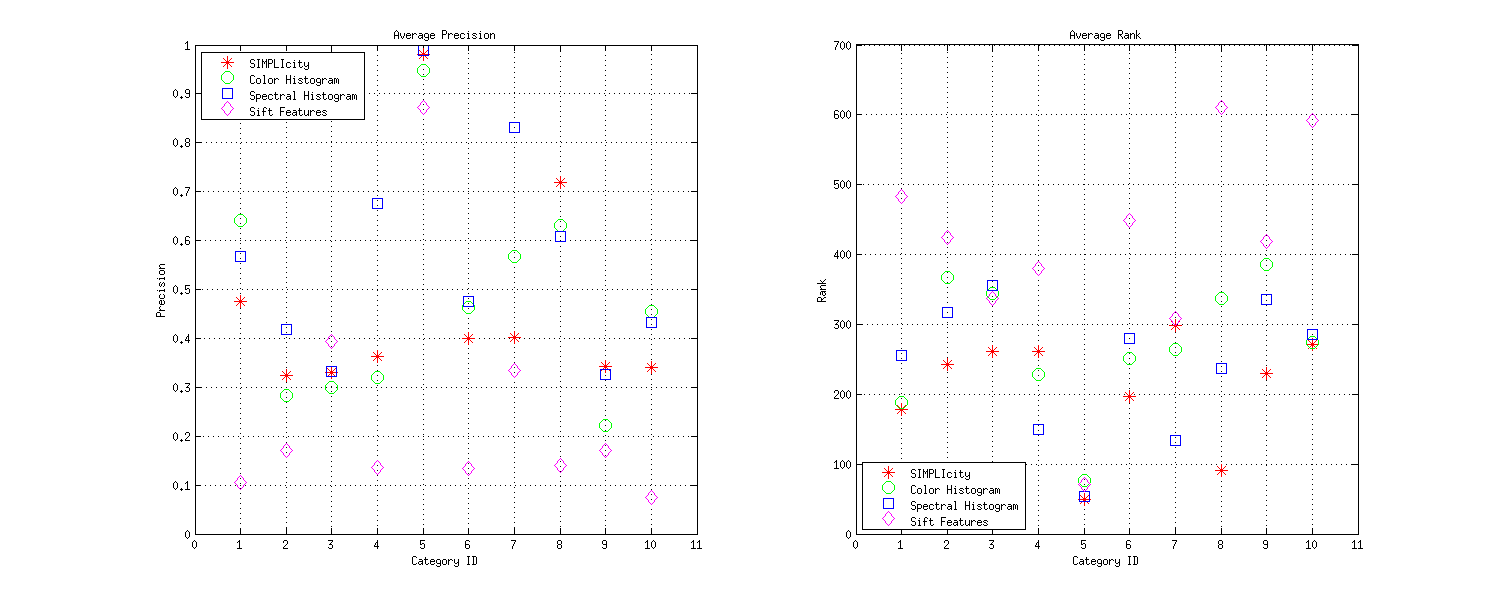
\includegraphics[totalheight=.30\textheight]{./Images/AllResults.png}
    \label{fig:res}
\end{figure}

The following are some good and bad examples of the PR obtained for each method in 
specific images. Figure \ref{fig:good} shows the PR obtained for image $\#401$ for the
color histogram and spectral histogram methods. In this case both obtain good PR plots, 
but the Spectral histogram method is better. 

\begin{figure}[h!]
    \centering
    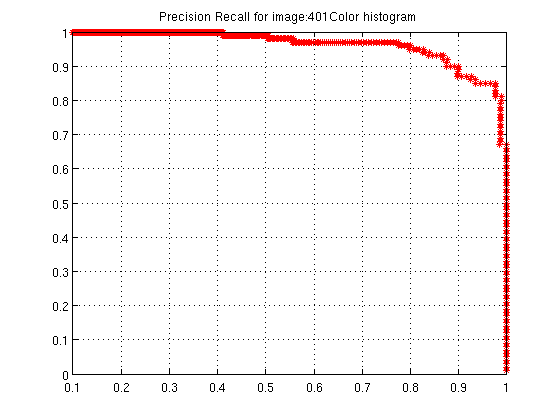
\includegraphics[totalheight=.24\textheight]{../Results/PR/GoodColor.png}
    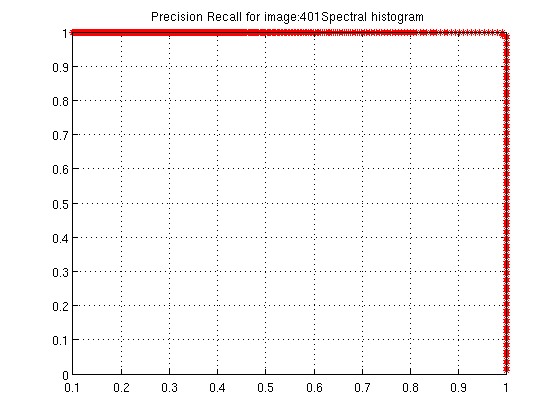
\includegraphics[totalheight=.24\textheight]{../Results/PR/GoodSpectral.png}
    \label{fig:good}
\end{figure}

Figure \ref{fig:bad} shows the PR obtained for image $\#361$ for Spectral and color histogram. This
is an example where the classification is bad. In this example both methods obtain similar
results. 
\begin{figure}[h!]
    \centering
    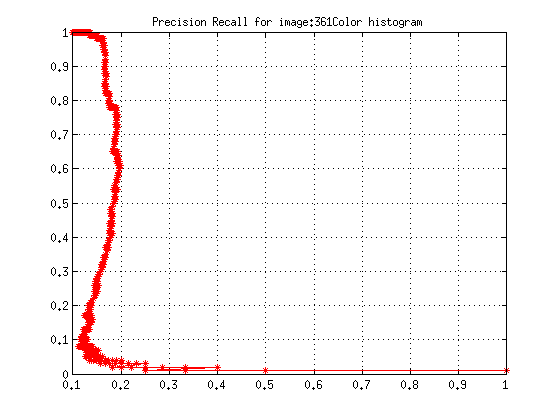
\includegraphics[totalheight=.24\textheight]{../Results/PR/BadColor.png}
    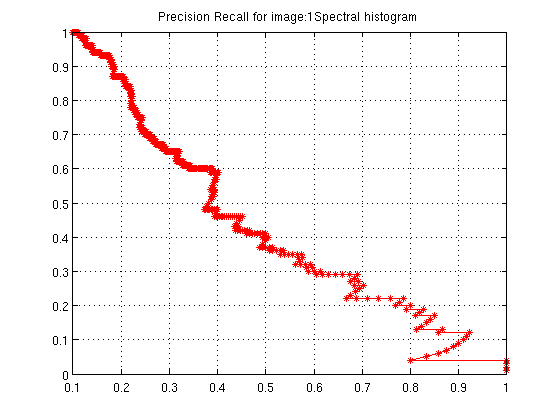
\includegraphics[totalheight=.24\textheight]{../Results/PR/BadSpectral.png}
    \label{fig:bad}
\end{figure}

Finally, figure \ref{fig:sgb} shows two PR curves obtained with the SIFT features method.
The first case is the image $\#481$ which obtains very good results. This image belongs
to the 5th category, which is mostly the only category where SIFT is better than SIMPLICITY.
The right plot of figure \ref{fig:sgb} shows the PR plot for image $\#331$ where it obtains very poor results.
\begin{figure}[h!]
    \centering
    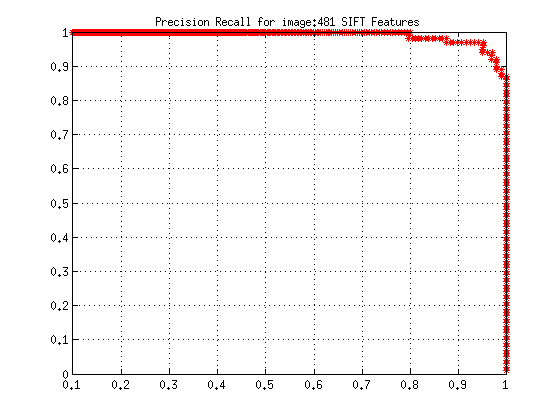
\includegraphics[totalheight=.24\textheight]{../Results/PR/GoodSIFT.png}
    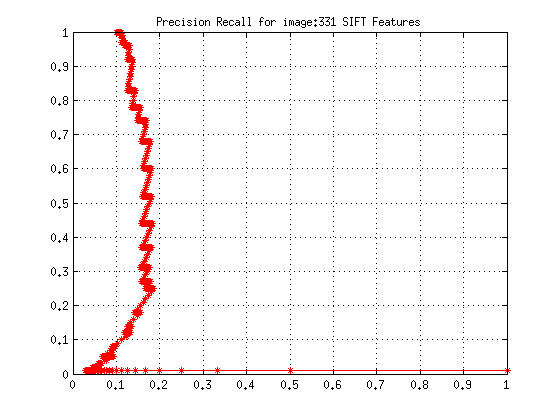
\includegraphics[totalheight=.24\textheight]{../Results/PR/BadSIFT.png}
    \label{fig:sgb}
\end{figure}

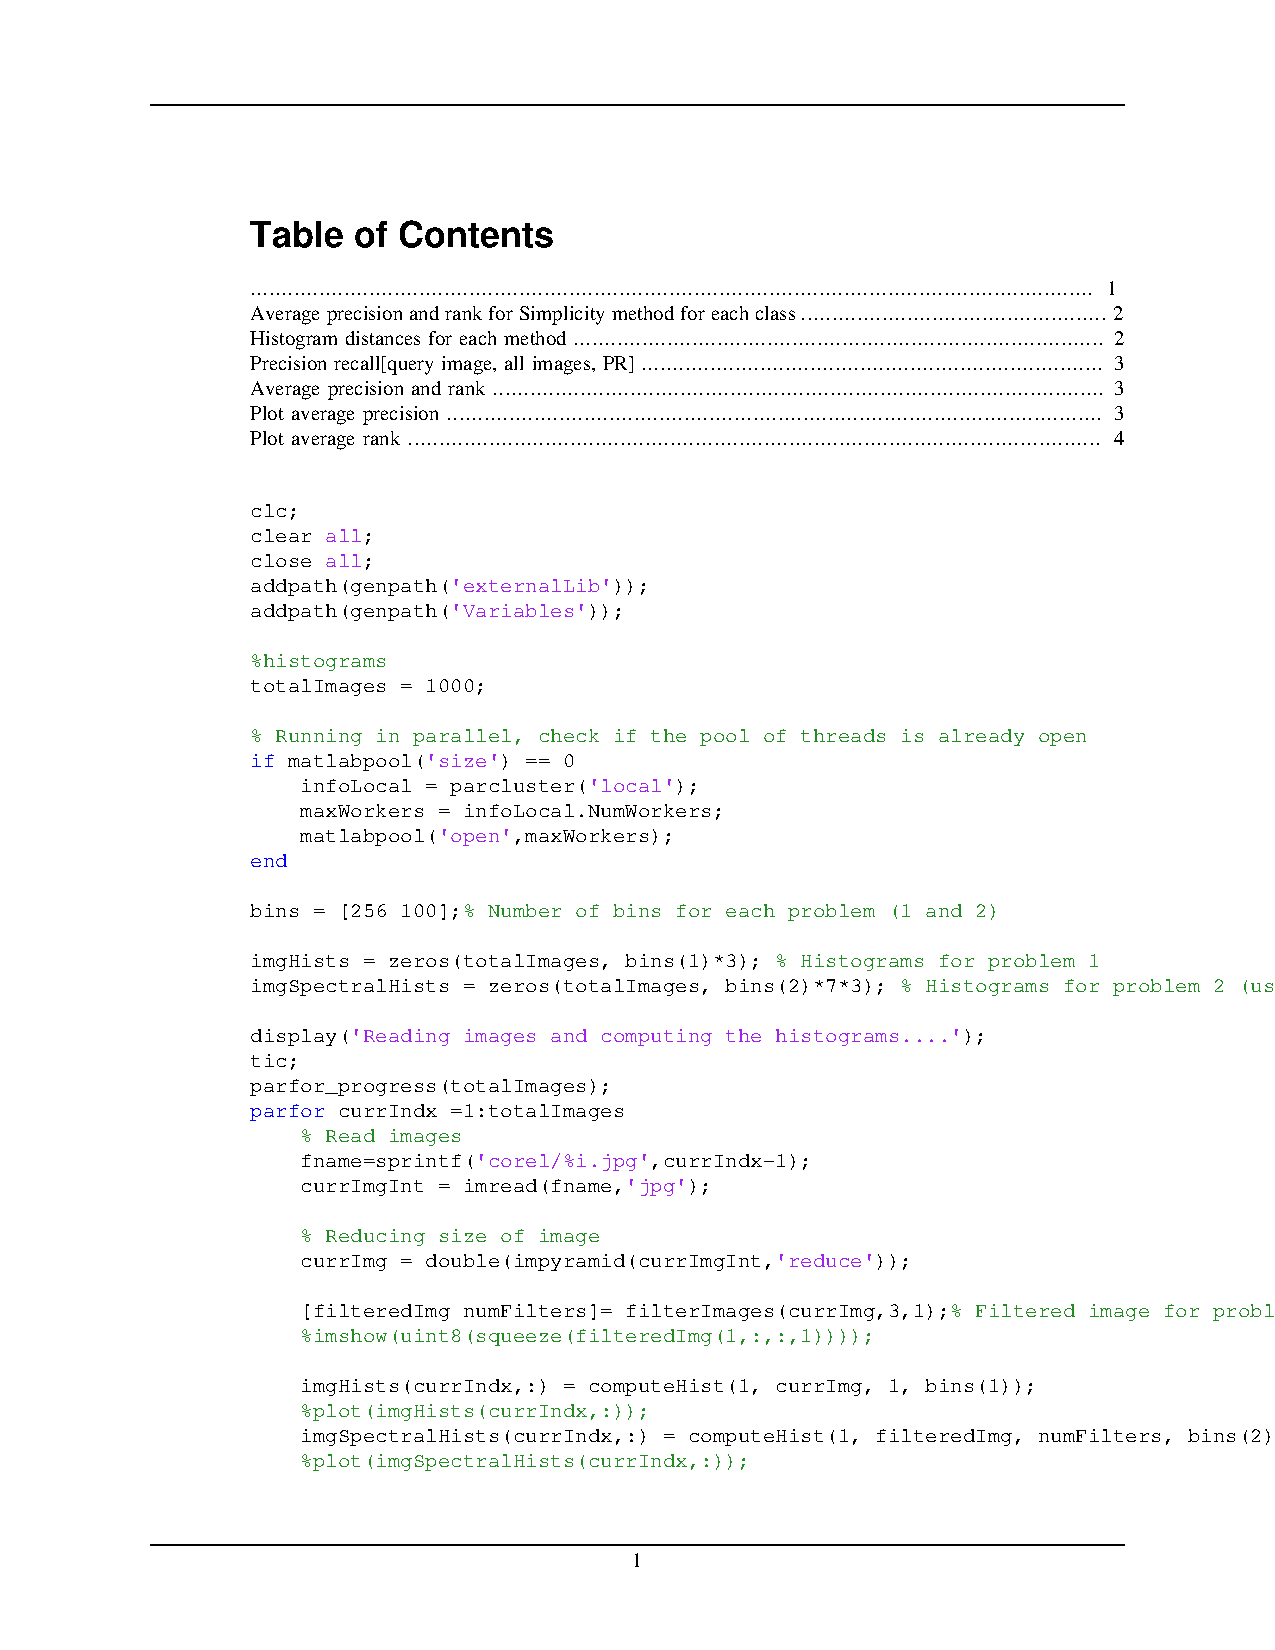
\includepdf[pages={1-15}]{Code.pdf}

\end{document}
